\documentclass[12pt]{article}
\usepackage[
    marginparwidth=2.5cm, marginparsep=3mm
]{geometry}                % See geometry.pdf to learn the layout options. There are lots.
\geometry{letterpaper}                   % ... or a4paper or a5paper or ... 
%\geometry{landscape}                % Activate for for rotated page geometry
%\usepackage[parfill]{parskip}    % Activate to begin paragraphs with an empty line rather than an indent
\usepackage{float}
\usepackage{graphicx}
\graphicspath{{images/}}
\usepackage{amsmath,amssymb,amsfonts,amsthm}
\usepackage{epstopdf}
\usepackage{epigraph}
\usepackage{url}
\usepackage{mathtools}
\usepackage{tikz-cd}
\usepackage{hyperref}
%\usepackage{cleveref}
\usepackage[linewidth=0.2mm]{mdframed}
\usepackage{marginnote}
\renewcommand*{\marginfont}{\footnotesize}
\reversemarginpar
\usepackage{listings}
\lstset{basicstyle=\ttfamily}

% Computer Concrete
%\usepackage{concmath}
%\usepackage[T1]{fontenc}

% Times variants
%
%\usepackage{mathptmx}
%\usepackage[T1]{fontenc}
%
%\usepackage[T1]{fontenc}
%\usepackage{stix}
%
% Needs to typeset using LuaLaTeX:
%\usepackage{unicode-math}
%\setmainfont{XITS}
%\setmathfont{XITS Math}

% garamond
%\usepackage[cmintegrals,cmbraces]{newtxmath}
%\usepackage{ebgaramond-maths}
%\usepackage[T1]{fontenc}

\DeclareGraphicsRule{.tif}{png}{.png}{`convert #1 `dirname #1`/`basename #1 .tif`.png}

\theoremstyle{plain}
\newtheorem{theorem}{Theorem}
\newtheorem{corollary}[theorem]{Corollary}
\newtheorem{lemma}[theorem]{Lemma}
\newtheorem{proposition}[theorem]{Proposition}
\newtheorem{conjecture}[theorem]{Conjecture}
\newtheorem{question}[theorem]{Question}
\newtheorem{exercise}[theorem]{Exercise}
\newtheorem{problem}[theorem]{Problem}
\newtheorem{definition}[theorem]{Definition}

\theoremstyle{definition}
\newtheorem{example}[theorem]{Example}
\newtheorem{todo}{TODO}

\theoremstyle{remark}
\newtheorem{remark}[theorem]{Remark}
\newtheorem{note}[theorem]{Note}

\newcommand*{\defeq}{\mathrel{\vcenter{\baselineskip0.5ex \lineskiplimit0pt
                     \hbox{\scriptsize.}\hbox{\scriptsize.}}}
                     =}
\newcommand{\N}{\mathbf N} 
\newcommand{\Q}{\mathbf Q} 
\newcommand{\R}{\mathbf R}

\DeclareMathOperator{\tr}{tr}
\DeclareMathOperator*{\sumtext}{sum}

\apptocmd{\lim}{\limits}{}{}
\apptocmd{\sum}{\limits}{}{}
\apptocmd{\prod}{\limits}{}{}
\apptocmd{\sumtext}{\limits}{}{}

\title{Neural Networks Notes}
\author{Nhan Trong}
\date{July 6, 2016---\today}                                           % Activate to display a given date or no date

\begin{document}
\sloppy
\maketitle

\epigraph{Pipey. \textit{Looks like you want to compress a movie file, can I help? You know with Pied Piper's revolutionary neural network optimized sharded data distribution system, it's just six clicks away, follow meeee!}}{Silicon Valley}

\tableofcontents % remember to compile twice to update table of contents

\part{Different Types of Neurons and Learning}

\begin{question}
How many other neurons does a neuron talk to? Do they change neighbours?
\end{question}

\begin{note}
``Goal of unsupervised learning: provides a compact, low-dimensional representation of the input,'' like Pied Piper's compression algorithm using neural networks!
\end{note}

\section*{Keywords}

Fruit flies, MNIST, TIMIT, linear, binary threshold, rectified / linear threshold, logistic, stochastic binary neurons, supervised, unsupervised, reinforcement learning.

\part{Neural Network Architectures}

\section*{Keywords}

Feed forward, recurrent, symmetrically connected neural network, perceptrons, convexity condition.

\part{Perceptron Learning Algorithm}

\begin{todo}
Proof of why perceptron learning works is very sketchy! Need more details.
\end{todo}

\section{Binary Threshold Neurons / McCulloch-Pitts}

Used in Perceptrons.

\begin{question}
Also called Linear Threshold Neurons?
\end{question}

\begin{definition}
First compute $z = w^T x$, then output $$y = \begin{cases}
1 \text{ if } z \geq 0 \\
0 \text{ otherwise,}
\end{cases}$$ representing ``all VS none'' activation.
\end{definition}

\begin{note}
Here we implicitly added the threshold as a bias unit: $w = (b, w_1, w_2, \ldots)$.
\end{note}

\begin{remark}
The function $y(z)$ is also called the Heaviside / unit step function.
\end{remark}

\begin{figure}[H]
\centering
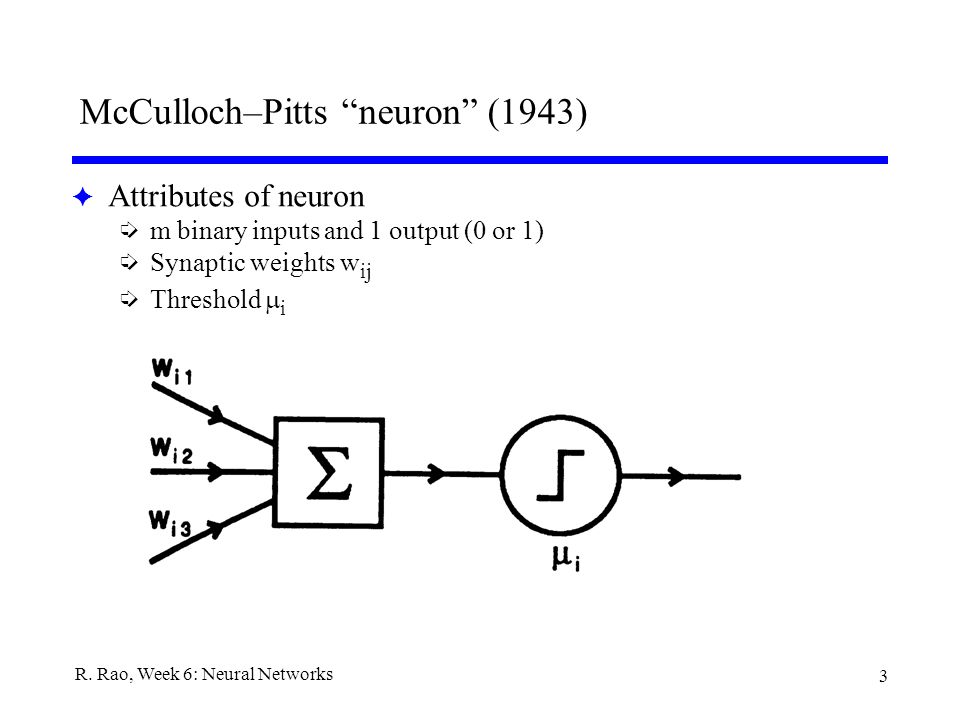
\includegraphics[width=1.0\textwidth]{mccullochpitts}
\end{figure}

\section{Limitations of the Binary Threshold Neuron}

\begin{proposition}
A single binary threshold neuron cannot learn the XOR function, because geometrically its truth table represented on a plane is not linearly separable.
\end{proposition}

\begin{figure}[H]
\centering
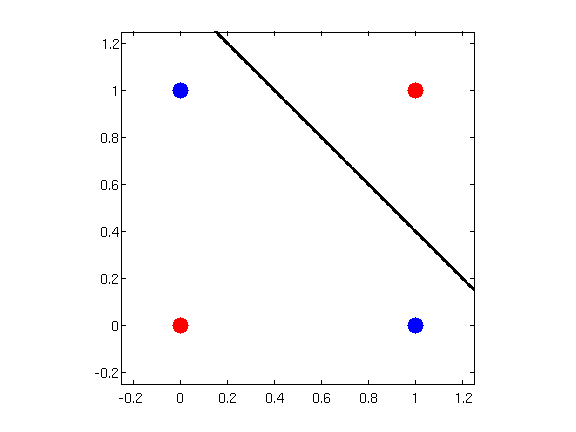
\includegraphics[width=1.0\textwidth]{linSepXor}
\end{figure}

\subsection{Group Invariance Theorem}

\begin{proposition}
Perceptrons can't learn patterns if they're subject to transformations that form a group, e.g. translations with wrap-around.
\end{proposition}

\begin{question}
Details?
\end{question}

\section*{Keywords}

Data space, weight space, Group Invariance Theorem.

\part{Linear Neuron Learning Algorithm}

\begin{definition}
Given a training case $x_n$ and a weight vector $w$, the neuron's estimate $y_n$ of the desired output is $$y_n = \sum_{i}^{} w_i x_{ni} = w^T x_n.$$ Define the cost function $E_n$ to be the squared difference error $$E_n = \frac{1}{2}(t_n - y_n)^2,$$ where $t_n$ is the target output, i.e. the ``ground truth'', and define the total error to be $$E = \sum_{n}^{} E_n.$$ Finally the goal of learning is to minimize $E$: $$\min_{w} E.$$
\end{definition}

\section{Delta Rule: Learning by Gradient Descent}

The error partials are 
$$\frac{\partial E}{\partial w_i} = \sum_n \frac{dE_n}{dy_n} \frac{\partial y_n}{\partial w_i} = - \sum_n (t_n - y_n) x_{ni}.$$
The Delta Rule / Gradient Descent says that we should change $w_i$ in the opposite direction as the change in error along $w_i$, give or take a learning rate $\alpha$:
$$\Delta w_i = - \alpha \frac{\partial E}{\partial w_i} = \sum_n \alpha (t_n - y_n) x_{ni},$$ i.e. $\alpha$ tells us how much to change, and the negative sign tells us which direction to go, namely the opposite direction. E.g. if $\frac{\partial E}{\partial w_i} > 0,$ that means the error goes up as $w_i$ increases, so we want to decrease $w_i$ to make it go down, and vice versa.

\section{Error Surface of a Linear Neuron}

\begin{question}
IIRC feature normalization should help with slow learning due to unscaled data? What about pathological cases like this?
\end{question}

\begin{figure}[H]
\centering
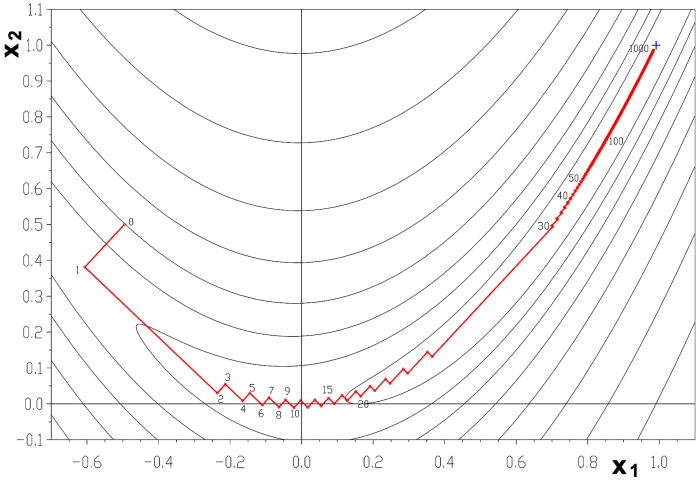
\includegraphics[width=1.0\textwidth]{slowlearrning}
\caption{Rosenbrock Valley.}
\end{figure}

\section*{Keywords}

Linear neurons / linear filters, iterative / computational VS analytic / mathematical approach, Delta Rule / Gradient Descent, batch VS online, error surface, extended weight space, Rosenbrock function.

\part{Logistic Neurons}

\section{Learning Rule}

\begin{definition}
The estimator for a logistic neuron is given by
$$y = \frac{1}{1 + e^{-z}}$$ where $z = w^T x.$ The function $y(z)$ is also known as a logistic / sigmoid function, and $z$ is sometimes called the logit. As before, the error is the squared difference
$$E = \frac{1}{2} \sum_n (t_n - y_n)^2.$$
\end{definition}

\begin{figure}[H]
\centering
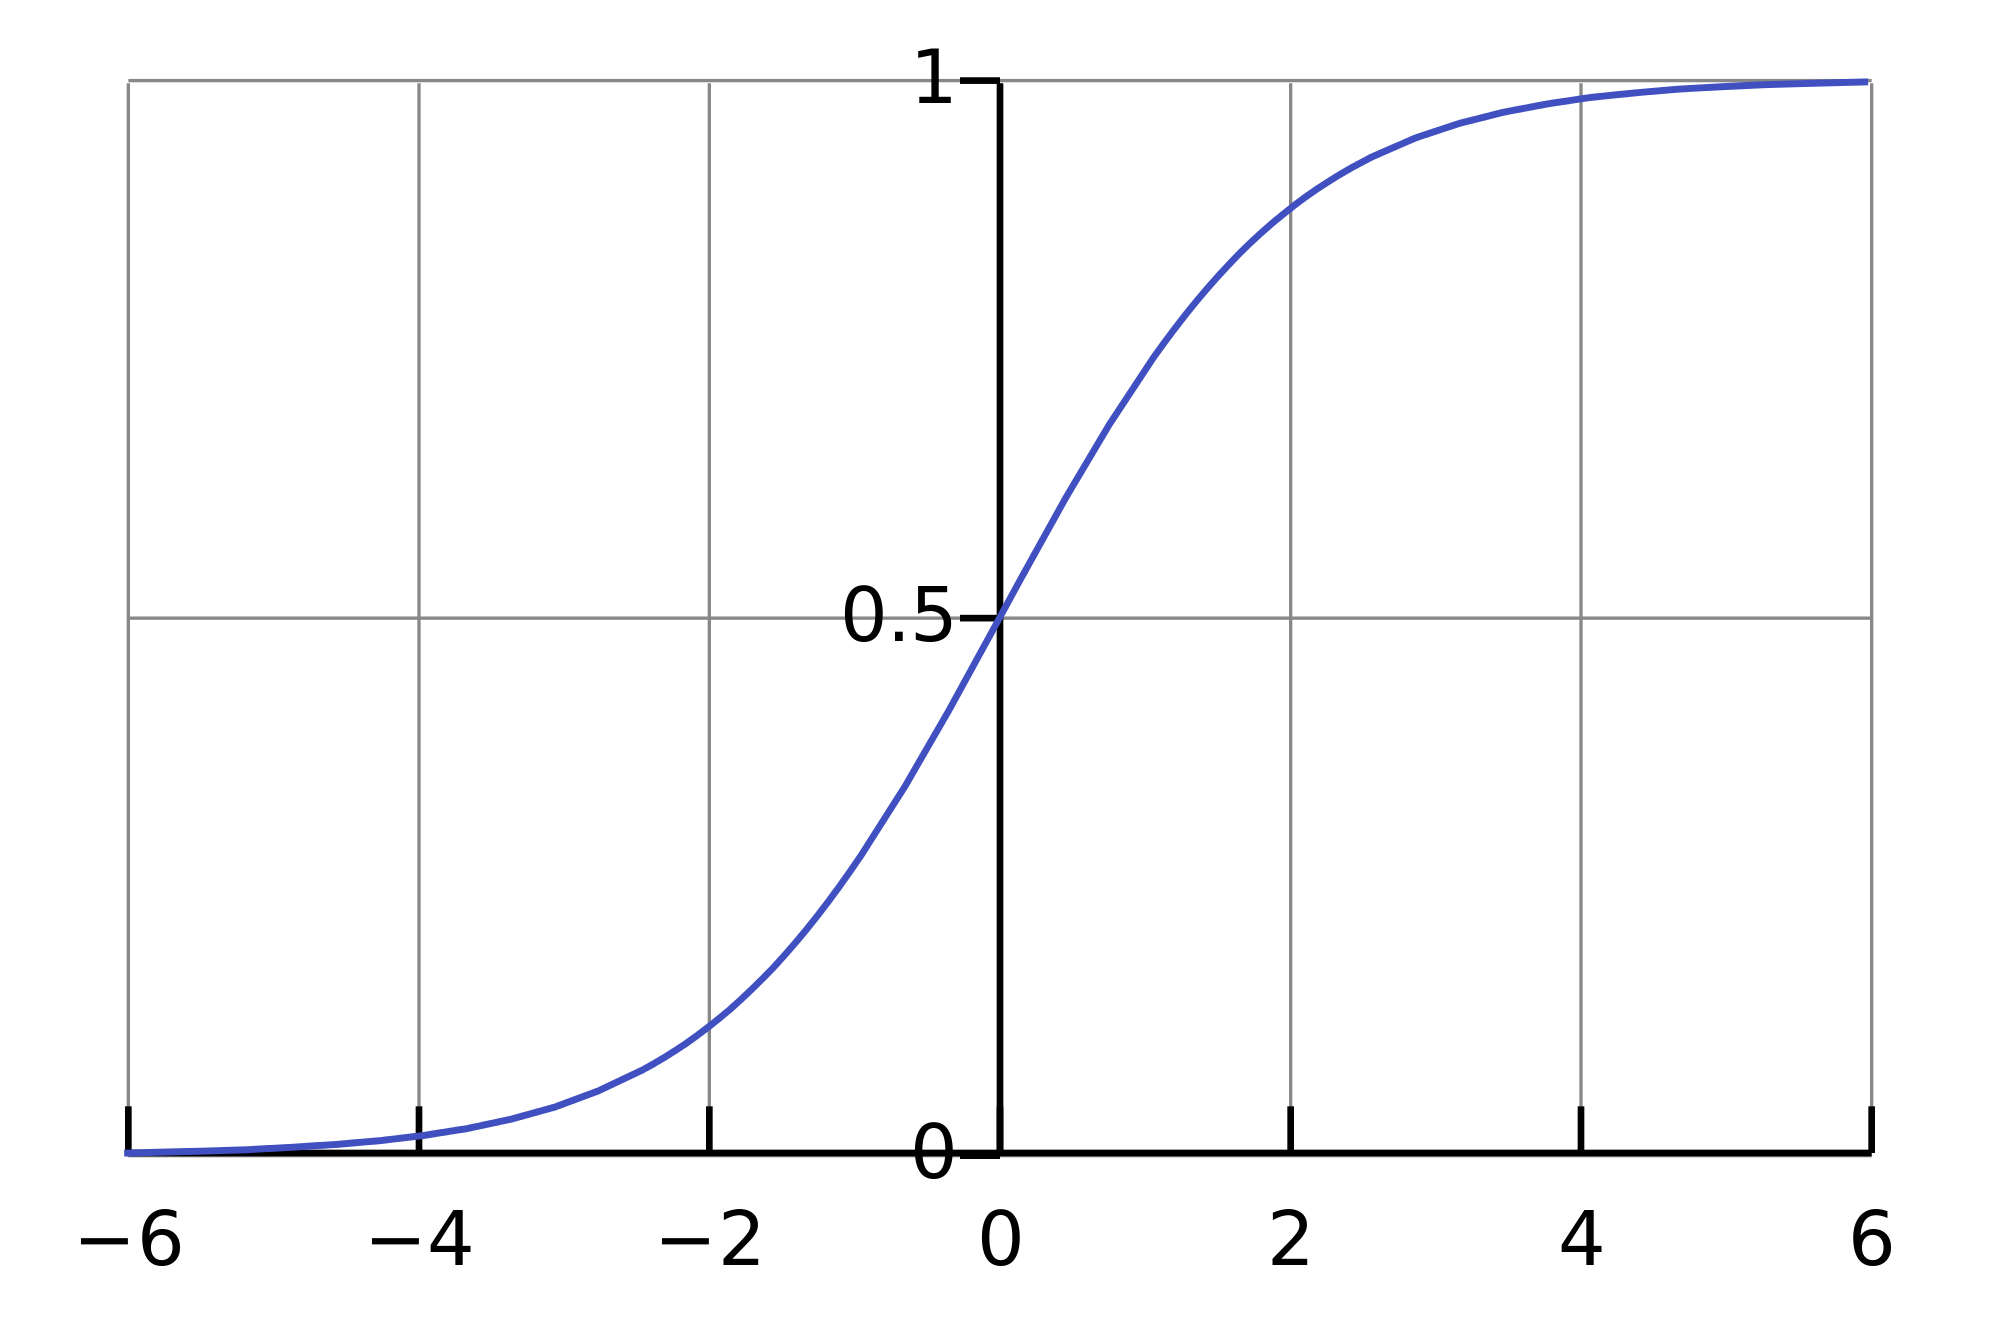
\includegraphics[width=.7\textwidth]{Logistic-curve}
\end{figure}

\begin{proposition}
\label{simpleerrorderivatives}
The estimator derivatives are
$$\frac{\partial y}{\partial w_i} = \frac{dy}{dz} \frac{\partial z}{\partial w_i} 
= y(1 - y) x_i,$$ and so the error derivatives are
$$\frac{\partial E}{\partial w_i} = \sum_n \frac{dE_n}{dy_n} \frac{\partial y_n}{\partial w_i} = - \sum_n (t_n - y_n)(1 - y_n) y_n x_{ni}.$$
\end{proposition}

\section{Learning with Hidden Units}

\subsection{Simplifying Notations}

\marginnote{Deliberately conflating a neuron $y_j$ with layer $j$.}
In a neural networking using logistic neurons with hidden layers, the neurons $y_n$ are arranged in layers, with neurons in each layer receiving input from every neuron in the layer below, and outputting to every neuron in the layer above it. To simplify notations, $y_i$ is used to denote any neuron in a fixed row $i$, and $y_j$ to denote any neuron in the layer $j$ above it.

The weights controlling how neurons in row $i$ act on neurons in row $j$ are $w_{ij}$, where $i$ ranges over the neurons in row $i$ and $j$ ranges over neurons in row $j$. Furthermore, $w_{ij}$ is also used to denote the weight of neuron $y_i$ on neuron $y_j$, so that e.g. the logit for neuron $y_j$ is $$z_j = w_{-} y_{-} + \cdots + w_{ij} y_{i} + \cdots + w_{-} y_{-},$$ where each unnamed $w_{-} y_{-}$ is a weight and neuron in row $i$, and we're only interested in the weight and neuron $w_{ij} y_{i}$, so we give them names $ij$ and $i$.

\begin{figure}[H]
\centering
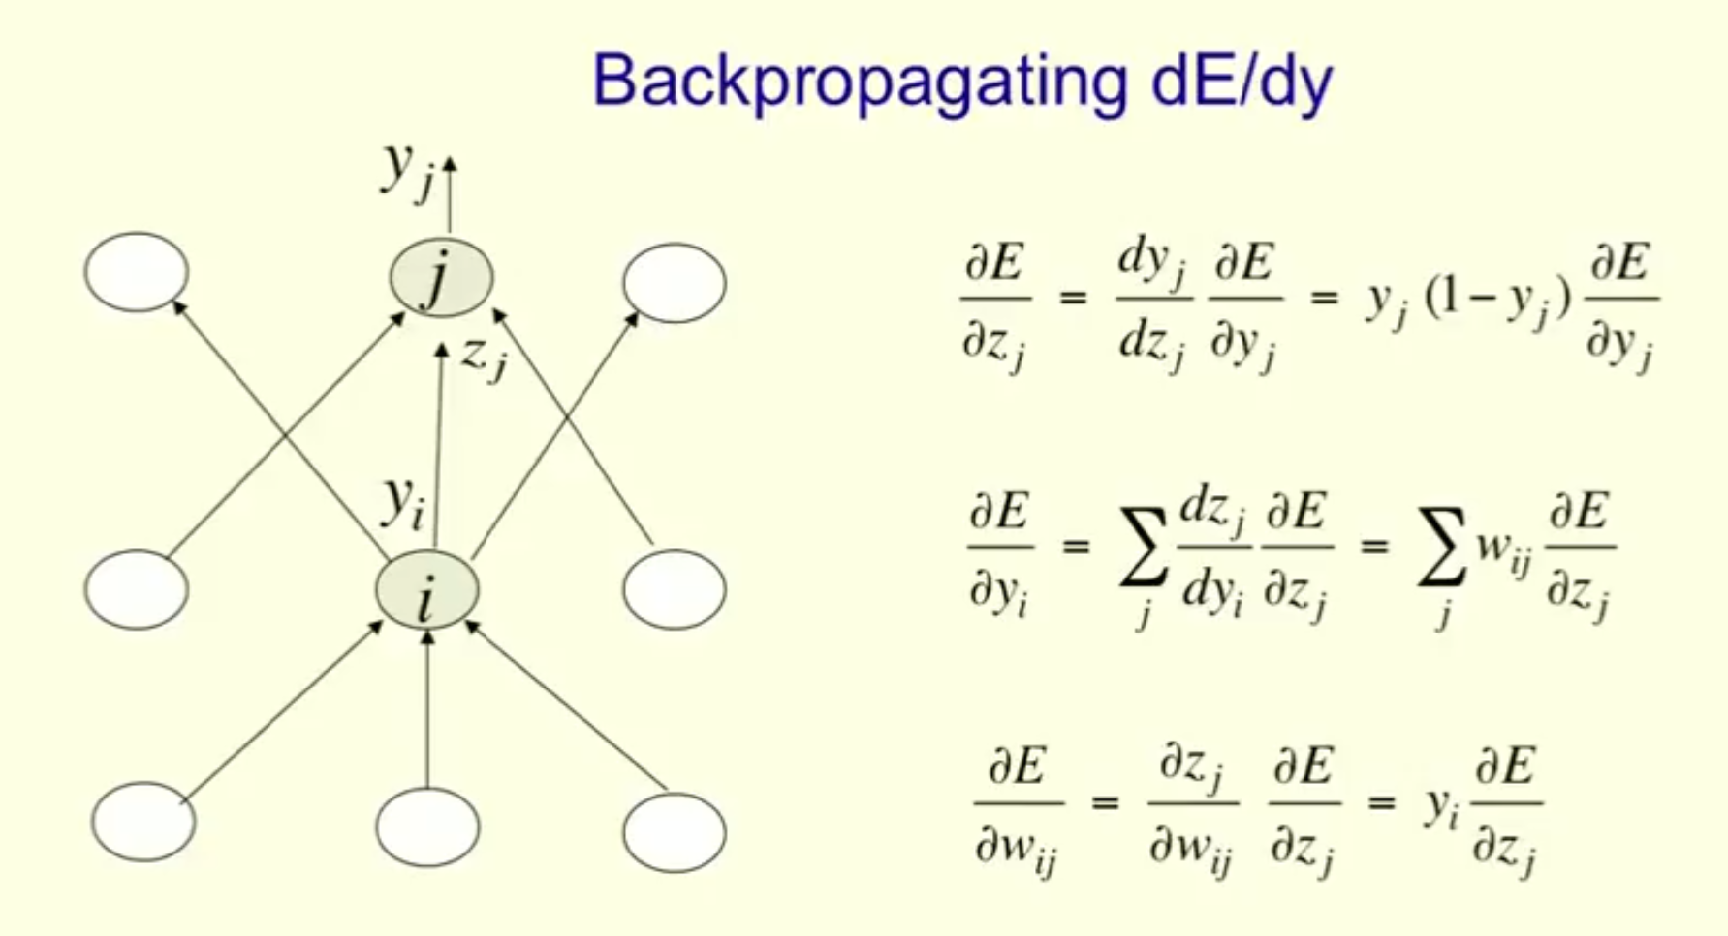
\includegraphics[width=1.0\textwidth]{backprop}
\caption{Model and main equations for Backpropagation.}
\end{figure}

\section{Backpropagation Algorithm}

\begin{mdframed}
Given an error $E$ and a training case $x = y_1,$ we want to compute the errors of $E$ due to $y_n$ for all neurons $y_n$, i.e. we want to compute $\frac{\partial E}{\partial w_{ij}}$ for all $ij$. With these partial derivatives calculated over all training cases, we can then apply Gradient Descent or some other optimization algorithm to \textit{compute} the minimum weights $W.$
\footnote{Keep in mind that there is a weight matrix $w$ for each pair of layers $i$ and $j,$ where each entry $w_{ij}$ corresponds to the connection between neuron $y_i$ in layer $i$ and neuron $y_j$ in layer $j.$ \\ Therefore the weights of all connections together form a three-dimensional matrix $W.$}
\end{mdframed}

\subsection{Analytic Solution vs Random Perturbation}

\marginnote{A kind of reinforcement learning.}
An alternative to using Backpropagation is to randomly perturb the weights and see how each change affects the error, but that's a lot slower than solving for the optimal solution analytically, since you have to test a single weight change on \textit{all} training cases to see if that change made an improvement on the error.

\subsection{Deriving the Error Derivatives}

\begin{definition}
For quick reference, once again the logit and estimator of neuron $y_j$ in layer $j$ are:
\begin{align*}
z_j &= w^T x = w_- y_- + \cdots + w_{ij} y_i + \cdots + w_- y_- \\
y_j &= \frac{1}{1 + e^{-z_j}}.
\end{align*}
And the total error of the neural network is:
$$E = \frac{1}{2} \sum_n (t_n - y_n)^2.$$
\end{definition}

\begin{mdframed}
\begin{proposition}
\marginnote{It's like a recursive Chain Rule.}
The error derivatives for a logistic neural network with hidden units are:
\begin{align}
\frac{\partial E}{\partial z_j} &= \frac{\partial E}{\partial y_j} \frac{dy_j}{dz_j} = y_j (1 - y_j)  \frac{\partial E}{\partial y_j} \\
\frac{\partial E}{\partial y_i} &= \sum_j \frac{\partial E}{\partial z_j} \frac{\partial z_j}{\partial y_i} = \sum_j w_{ij} \frac{\partial E}{\partial z_j} \\
\frac{\partial E}{\partial w_{ij}} &= \frac{\partial E}{\partial z_j} \frac{\partial z_j}{\partial w_{ij}} = y_i \frac{\partial E}{\partial z_j}.
\end{align}
\end{proposition}
\end{mdframed}

These equations are simple applications of the Chain Rule. But what could they possibly mean?!

\subsection{Meaning of the Error Derivatives and How to use them}

At layer $i$, consider $E$ as a function of the $z_j$'s in layer $j$. Since $z_j$ depend on $y_i$, by the Chain Rule we have the second equation: 
$$\frac{\partial E}{\partial y_i} = \sum_j \frac{\partial E}{\partial z_j} \frac{\partial z_j}{\partial y_i} = \sum_j w_{ij} \frac{\partial E}{\partial z_j}.$$ 
To calculate $ \frac{\partial E}{\partial z_j}$, we use equation (1): 
$$\frac{\partial E}{\partial z_j} = \frac{\partial E}{\partial y_j} \frac{dy_j}{dz_j} = y_j (1 - y_j)  \frac{\partial E}{\partial y_j},$$
which requires $\frac{\partial E}{\partial y_j},$ so we use equation (2) again to level up, and so on until the top output layer.

In practice we'd start at the top and calculate down, and along the way down we use the third equation to calculate $\frac{\partial E}{\partial w_{ij}}$. Once we have all of those we use the Delta Rule to calculate the necessary weight changes: $$\Delta w_{ij} = - \alpha \frac{\partial E}{\partial w_{ij}}.$$

\subsection{Optimization Issues}

\begin{question}
How often to update weights: online, full batch, mini batch.
\end{question}

\begin{question}
How much to update weights via $\alpha$ learning rate: fixed, adaptive, adaptive per connection, alternatives to Steepest Descent.
\end{question}

\subsection{Generalization Issues / overfitting}

\marginnote{Hey, polynomial approximation!}
Ways to reduce overfitting: weight decay, weight sharing, early stopping, model averaging, Bayesian fitting of neural nets, dropout, generative pre-training.

\section*{Keywords}

Sigmoid function, logit, Backpropagation Algorithm, weight perturbation, evolution, overfitting, sampling error.

\section{Application: learning to predict the next word}

\begin{example}
Learn $ArB$ to guess $B$ given $A$ and $r$.
\end{example}

\begin{figure}[H]
\marginnote{Why 6 neurons? Cross validate to choose the best number?}
\centering
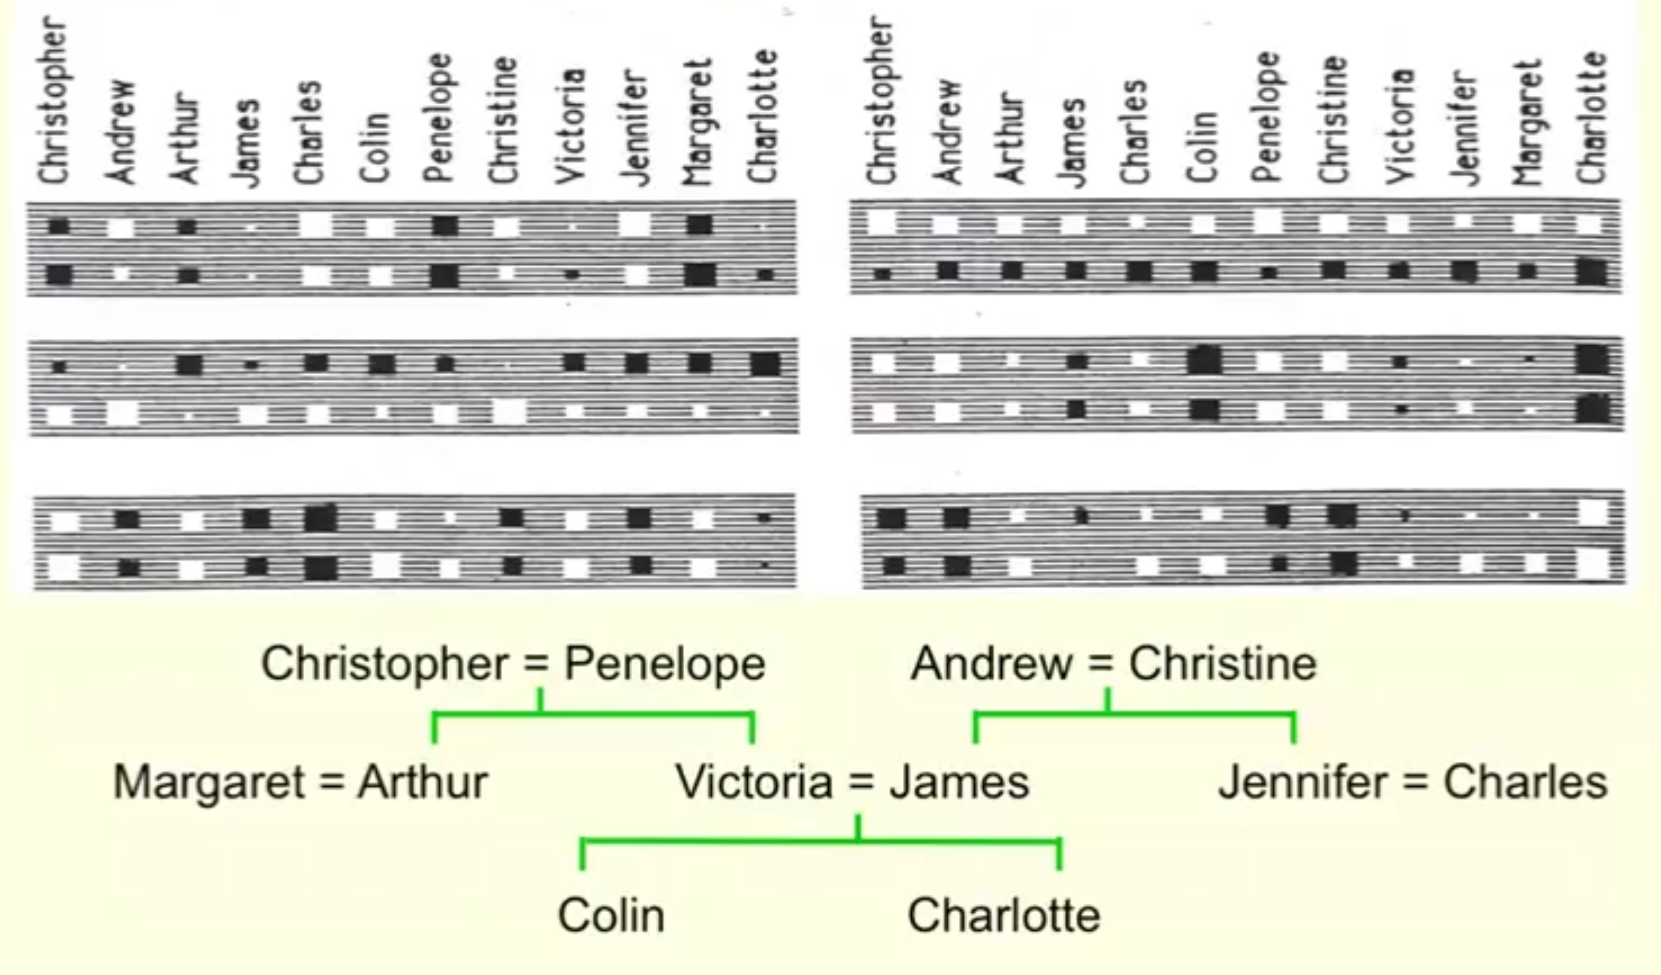
\includegraphics[width=1.0\textwidth]{familytree}
\caption{Six-neuron hidden layer for distributed encoding of Person 1. The 24 squares in each neuron are the weights of its inputs, corresponding to the 24 English and Italians.}
\end{figure}

\begin{example}
Another application of $ArB$ is to guess the probability of $ArB$ being correct given $A, r,$ and $B.$ Need both correct and incorrect training cases for learning.
\end{example}

\section{Digression: Philosophy of Learning}

Feature theory: a concept is a set of semantic features. Structuralist theory: meaning of a concept lies in its relationships to other concepts. 

Hinton: why not both?

\begin{question}
How to implement relational knowledge in a neural net? Maybe many neurons per concept and one neuron reused in multiple concepts.
\end{question}

\begin{question}
Why not all neurons in all concepts? Maybe cause then you'd have no relations? Kinda woolly at the moment.
\end{question}

\section{Digression: Softmax Output Function and Cross-Entropy Cost Function}

\begin{definition}
A softmax group $G$ is a group of output neurons whose outputs use the softmax activation function defined by $$y_i = \frac{e^{z_i}}{\sum\limits_{j\in G} e^{z_j}},$$ so that the outputs sum to $1.$ The cost function is given by $$C = - \sum_j t_j \log y_j.$$
\end{definition}

\begin{figure}[H]
\centering
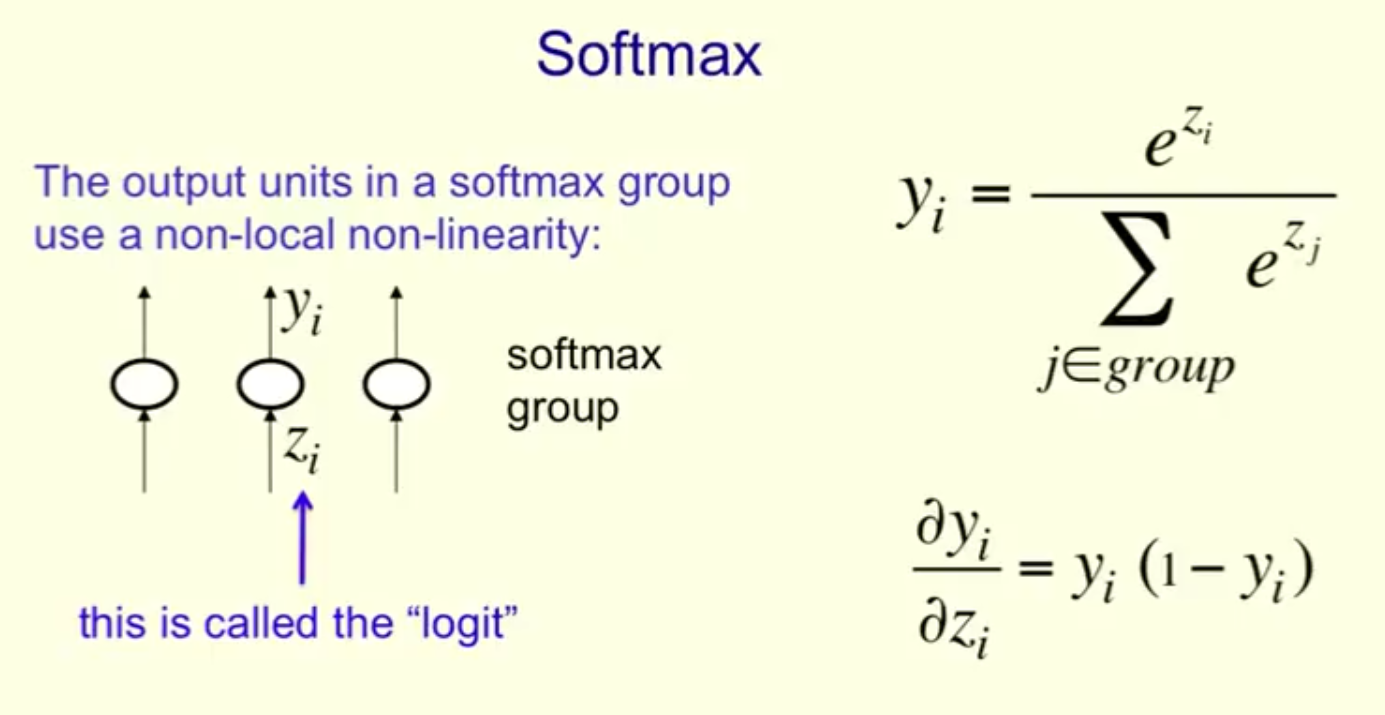
\includegraphics[width=1.0\textwidth]{softmaxgroup}
\end{figure}

\begin{mdframed}
\begin{proposition}
By the Quotient Rule, the derivatives are
\begin{align*}
\frac{\partial y_i}{\partial z_i} &= y_i(1 - y_i) \\
\frac{\partial y_i}{\partial z_j} &= -y_i y_j,
\end{align*}
or more fancy-like using the Kronecker Delta:
$$\frac{\partial y_i}{\partial z_j} = y_i(\delta_{ij} - y_j).$$
\end{proposition}
\end{mdframed}

\begin{mdframed}
\begin{proposition}
The derivatives of the cost function are:
$$\frac{\partial C}{\partial z_i} = y_i - t_i.$$
\end{proposition}
\end{mdframed}

\begin{proof}
Apply the Chain Rule:
$$\frac{\partial C}{\partial z_i} = - \sum_j t_j \frac{\partial \log y_j}{\partial z_i} = - \sum_j t_j \frac{\partial \log y_j}{\partial y_j} \frac{\partial y_j}{\partial z_i}.$$
Using our formula for $\frac{\partial y_j}{\partial z_i},$ we get 
$$\frac{\partial C}{\partial z_i} = - \sum_j \frac{t_j}{y_j} y_j(\delta_{ij} - y_i) = - \sum_j t_j (\delta_{ij} - y_i).$$
Recall that this is a multiclass classification problem, and so exactly one of the $t_j$'s is 1 and the rest are zero. Therefore:
$$\frac{\partial C}{\partial z_i} = - t_i (1 - y_i) + \sum_{j\neq i} t_j y_i = - t_i + y_i \sum_j t_j = y_i - t_i.\qedhere$$
\end{proof}

\subsection{Application: Multiclass Classification using Softmax and Cross Entropy}

Suppose an input $x$ belongs to class $i \in G.$ That means $t_i = 1$ and $t_j = 0$ for all other $j \in G.$ It also means that $y_i$---which represents the probability of the input belonging to class $i$---should be high, and the cost $$\marginnote{Why $\log$? Maybe cause it gives nice derivatives like $\frac{\partial C}{\partial z_i} = y_i - t_i.$}
C = - \sum_j t_j \log y_j = - \log y_i$$ encapsulates that idea: if $y_i$ is high, then we've guessed correctly and $C$ is low; otherwise $y_i$ is low, and we've guessed incorrectly and $C$ should be high---hence the negative sign.

\begin{note}
\marginnote{Ah, this is why.}
The reason we use $\log$ is that when the answer is $t_i = 1$, and we guess $y_i$ very close to zero, i.e. we've guessed very wrong, we want the cost to be very high, and we can see that from the graph of log: when $y_i$ is close to zero, $\log y_i$ is very negative and so $- \log y_i$ is very large, i.e. it's a big cost. And vice versa, if the answer is $1$ and we guess close to 1, then the cost is very nearly zero.
\end{note}

\begin{figure}[H]
\centering
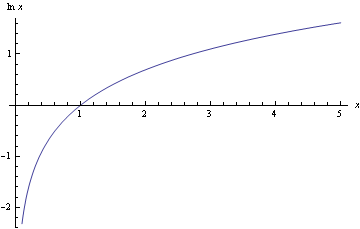
\includegraphics[width=0.7\textwidth]{figure_logarithmic_function}
\caption{Natural log}
\end{figure}

\begin{question}
What happens when $t_i = 0$, and we guess right with $y_i$ close to zero, or we guess wrong with $y_i$ close to one? The cost function $C$ seems to ignore those guesses. Shouldn't we punish those neurons that produce false positives and award ones that produce true negatives?
\end{question}

\section{Application: Speech Recognition}

\epigraph{\textit{People use their understanding of the meaning of the utterance to hear the right words. We do this unconsciously when we wreck a nice beach.}}{Geoffrey Hinton}

Speech recognizers have to know which words are likely to come next and which are not. 

\subsection{Trigram method}

Take a huge amount of text and count frequencies of all triples of words. Use these frequencies to calculate 
$$\frac{p(c|a,b)}{p(d|a,b)} = \frac{\mathrm{count}(abc)}{\mathrm{count}(abd)}.$$

Fall back to digram if trigram frequencies too low.

\begin{note}[Drawbacks]
Trigram doesn't understand similarity between words.
\end{note}

\begin{todo}
Need to do extra readings on the rest of the speech recognition lectures. Not a lot of details there.
\end{todo}

\epigraph{\textit{I will travel across the land,\\
Searching far and wide,\\
Each pokemon to understand\\
The power that's inside.\\
Pokemon! Gotta catch 'em all!
}}{Pokemon}

\part{Assignment 1: Learning Distributed Word Representations}

\begin{note}
Gonna use the Winter 2015 version of CSC321 cause they use Python instead of MATLAB.
\end{note}

\begin{problem}
Predict a word given a sequence of preceding words. Will need to build a neural net that can represent words well.
\end{problem}

\begin{figure}[H]
\centering
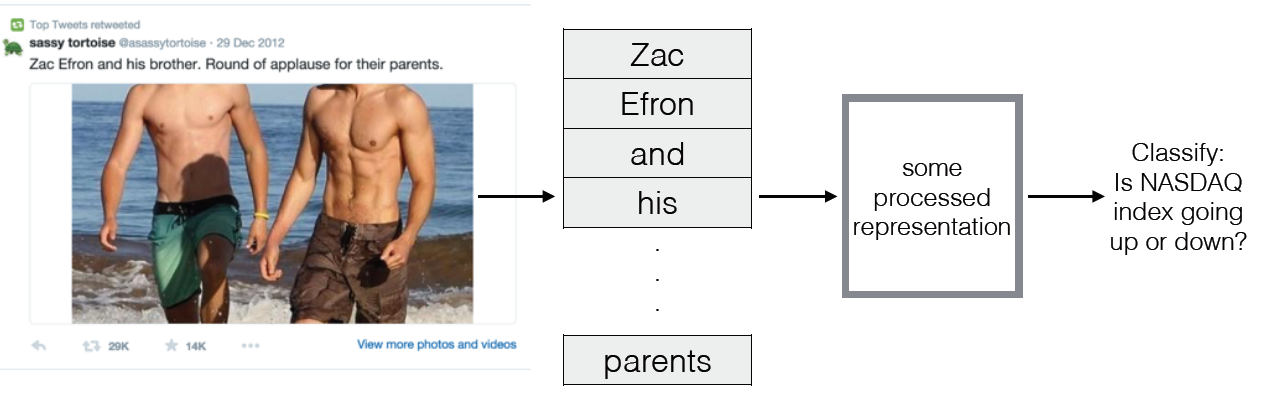
\includegraphics[width=1.0\textwidth]{zacefron}
\caption{Funny slide from handout.}
\end{figure}

\section{Network Architecture / Language Model}

Let $K = 250$ be the number of words in our dictionary, $D = 16$ be the number (also called the Embedding Dimension) of neurons for each word in the Embedding Layer, and let $H = 180$ be the number of neurons in the Hidden Layer. Note that the final output layer has $K$ neurons, with each output $y_k$ corresponding to the probability that the $k$-th word is the answer we're looking for, i.e. the $k$-th word is the word following the three input words.

\begin{figure}[H]
\centering
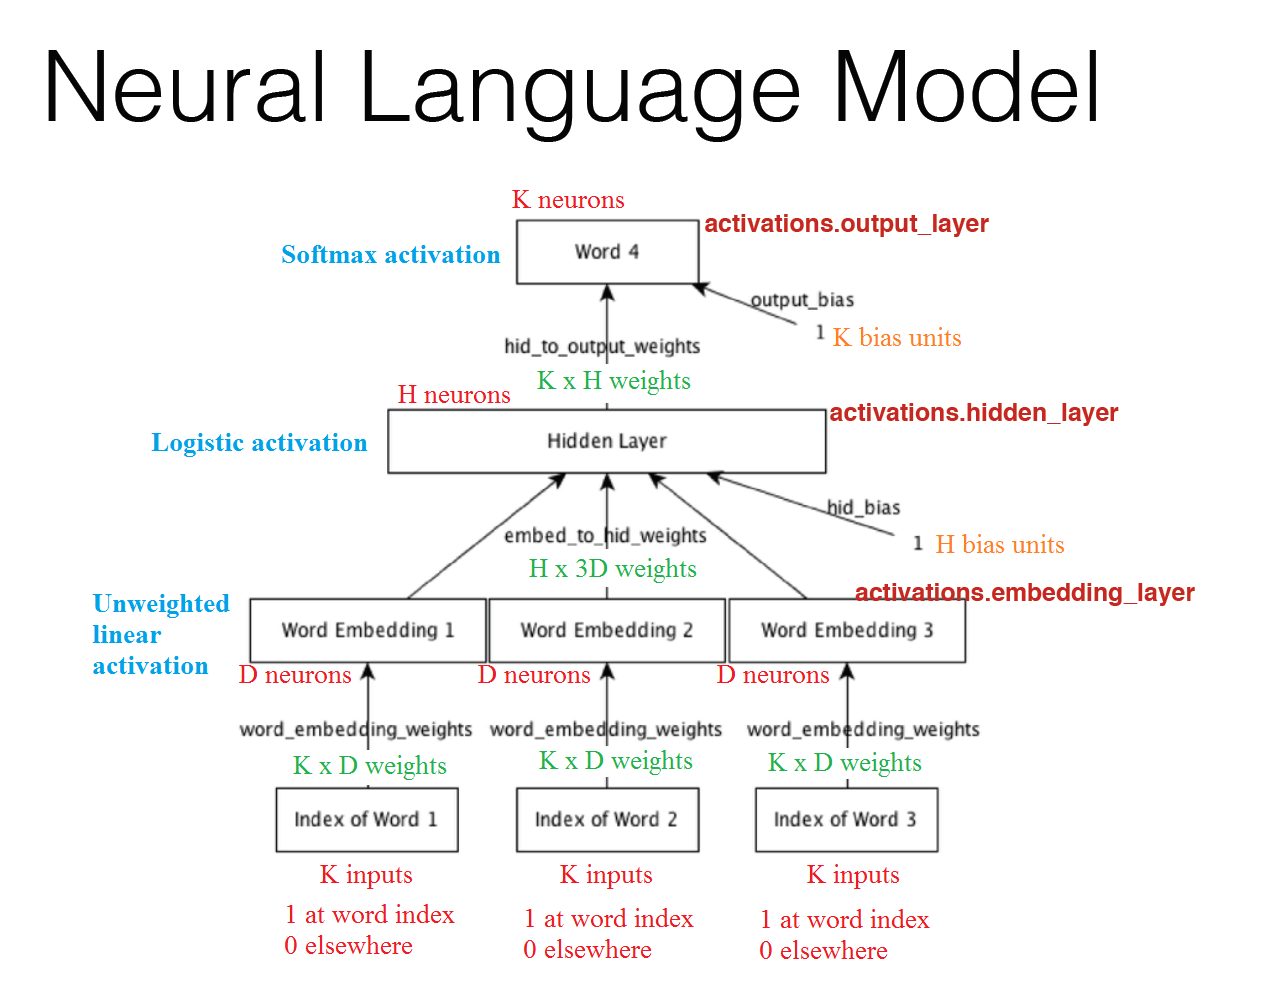
\includegraphics[width=1.0\textwidth]{neuralnetlanguagemodel}
\caption{Note that for implementation reasons \lstinline|embed_to_hid_weights| and \lstinline|hid_to_output_weights| are transposed, so you have $H \times 3D$ and $K \times H$ matrices instead of $3D \times H$ and $H \times K$.}
\end{figure}

\marginnote{An example of trade off between time (spent training the parameters) and space (to store the full lookup table).}
In the word embedding layer, we can just train one embedding model instead of three, one for each word. So in total the trainable parameters in the network is $$KD + (3DH + H) + (HK + K) = 58070,$$ with $H$ extra bias parameters for the hidden layer and $K$ bias parameters for the output layer. On the other hand, if we wanted to store all $4$-gram frequencies explicitly, then we'd need $$K^4 = 250^4 = 3906250000$$ entries in the lookup table.

\section{Mini-batch Backpropagation}

The general backpropagation algorithm remains the same, but since our architecture is made up of different kinds of neurons (using different activation functions: unweighted linear in the embedding layer, logistic in the hidden layer, and softmax in the output layer) our derivatives are slightly different. In addition, the starter assignment code uses mini-batch, so we'll also show vectorized implementations of the derivatives.

\subsection{Output Layer}

Let $y_j$ be a neuron in the output layer and $z_j$ be its logit. Then the loss derivatives are the same as before:
$$\frac{\partial C}{\partial z_j} = y_j - t_j.$$
We can denote the matrix form as a row vector\marginnote{It's often pretty useful to check matrix dimensions, so we'll denote them by $\sim$.}
$$\frac{\partial C}{\partial Z_j} = Y_j - T_j \sim 1 \times K$$
of length $K,$ where the subscript just tells us which layer it is, in this case $j$ for output. Mini-batch requires that we calculate this derivative for $m = 100$ training cases, say, so the loss derivative 
$$\frac{\partial C}{\partial Z_j} = Y_j - T_j \sim m \times K$$ 
is in fact an $m \times K$ matrix, where $K = 250$ is the number of neurons in the output layer, which is also the number of words in our dictionary.

\subsection{Hidden Layer}

Let $y_h$ be a neuron in the hidden layer, $z_h$ be its logit, and $w_{jh}$ be its weight to one of the output neurons $y_j$. In particular we have
\begin{align*}
z_j &= \sum_h w_{jh} y_h\\
y_h &= \frac{1}{1 + e^{-z_h}}\\
z_h &= \sum_e w_{he} y_e
\end{align*}
where $y_e$ and $w_e$ are some neuron and its weight in the embedding layer. Then
$$\frac{\partial C}{\partial z_h} = \frac{\partial C}{\partial y_h} \frac{\partial y_h}{\partial z_h},$$
and apply the Chain Rule, remembering that all the $z_j$'s in the output layer depend on $y_h$:
$$\frac{\partial C}{\partial z_h} = \frac{\partial y_h}{\partial z_h} \sum_j \frac{\partial C}{\partial z_j} \frac{\partial z_j}{\partial y_h} = y_h (1 - y_h) \sum_j w_{jh} \frac{\partial C}{\partial z_j}.$$ Here we also used a very nice and useful derivative so it's worth writing down:
\begin{mdframed}
\begin{proposition}
\marginnote{Sometimes we'll also confuse $d$ with $\partial.$}
If $y = \frac{1}{1 + e^{-z}}$, then $$\frac{\partial y}{\partial z} = y (1 - y).$$
\end{proposition}
\end{mdframed}

Back on topic: let $W_h$ be the $K \times H$ weight matrix from the hidden layer to the output layer, so e.g. the first column of $W_h$ would be weights over the hidden layer neurons going into neuron 1 in the output layer. Let $Y_h$ be the $m\times H$ matrix of activations of the hidden layer for the $m$ mini-batch, so e.g. the first row of $Y_h$ contains the $y_h$ values of the hidden layer neurons on the first training case. Then the matrix form of $\frac{\partial C}{\partial z_h}$ is
$$\frac{\partial C}{\partial Z_h} = Y_h * (1 - Y_h) * \left(\frac{\partial C}{\partial Z_j}W_h\right) \sim m \times H,$$
where $*$ denotes element-wise multiplication.

The derivatives of $C$ with respect to the hidden to output weights are
$$\frac{\partial C}{\partial w_{jh}} = \frac{\partial C}{\partial z_j} \frac{\partial z_j}{\partial w_{jh}} = y_h \frac{\partial C}{\partial z_j}.$$
In matrix form, this becomes
$$\frac{\partial C}{\partial W_h} = \frac{\partial C}{\partial Z_j}^T Y_h \sim K \times H.$$
\marginnote{Sanity check: $\frac{\partial C}{\partial W_h}$ is $K \times H,$ the same size as $W_h.$}This last formula needs a bit of explanation: recall that $\frac{\partial C}{\partial Z_j}$ is an $m\times K$ matrix, and that $Y_h$ is an $m\times H$ matrix. Therefore the entries of $\frac{\partial C}{\partial W_h}$ are of the form 
$$\left(\frac{\partial C}{\partial W_h}\right)_{jh} = \sum_m y_h \frac{\partial C}{\partial z_j},$$
i.e. we're summing all the partial derivatives $\frac{\partial C}{\partial w_{jh}}$ over the mini-batch. This is because when we do Gradient Descent, the Delta Rule says that
$$\Delta w_{jh} = - \alpha \frac{\partial C}{\partial w_{jh}}$$
for one training case, so the change in $w_{jh}$ over all training cases is
$$\Delta w_{jh} = - \alpha \sum_m \frac{\partial C}{\partial w_{jh}}.$$

\subsection{Hidden Layer Bias Units}

Let $b_h$ be the bias unit in the hidden layer going into neuron $y_j$ in the output layer. Then 
$$\frac{\partial C}{\partial b_h} = \frac{\partial C}{\partial z_j} \frac{\partial z_j}{\partial b_h} = \frac{\partial C}{\partial z_j},$$
since $\frac{\partial z_j}{\partial b_h} = 1.$ Similar to the weight derivatives, we also want to sum these over the $m$ training cases, so
$$\frac{\partial C}{\partial b_h} = \sum_m \frac{\partial C}{\partial z_j},$$ which in matrix form is
$$\frac{\partial C}{\partial B_h} = \left(\sumtext_\text{rows}\frac{\partial C}{\partial Z_j}\right)^T \sim K \times 1,$$
where $\sumtext_\text{rows} A$ sums a matrix $A$ over its rows, so in particular $\sumtext_\text{rows} A$ is a row vector.\footnote{Similarly $\sumtext_\text{cols} A$ is a column vector. In NumPy this is \lstinline|sum(A, 0)| and \lstinline|sum(A, 1)|, respectively.}

\begin{note}
An alternative to treating bias units separately from normal neurons is to add a constant feature 1 in each input layer going in to the next layer.
\end{note}

\subsection{Embedding Layer}

Similar to the previous layer, let $y_e$ be a neuron in the embedding layer, $z_e$ be its logit, $w_{he}$ be its weight to neuron $y_h$ in the hidden layer. There is one difference: for reasons still unclear to me in this layer the starter code uses a linear activation function:\marginnote{Question. Why is this better than other activation functions?} $$y_e = z_e = \sum_i w_i y_i,$$ where $i$ ranges over the neurons per context word in the input layer. In particular this means $\frac{\partial y_e}{\partial z_e} = 1,$ and so
$$\frac{\partial C}{\partial z_e} = \frac{\partial C}{\partial y_e} \frac{\partial y_e}{\partial z_e} = \sum_h \frac{\partial C}{\partial z_h} \frac{\partial z_h}{\partial y_e} = \sum_h w_{he} \frac{\partial C}{\partial z_h}.$$
In matrix form this is
$$\frac{\partial C}{\partial Z_e} = \frac{\partial C}{\partial Z_h} W_e \sim m \times 3D.$$

The weight derivatives are
$$\frac{\partial C}{\partial w_{he}} = \frac{\partial C}{\partial z_h} \frac{\partial z_h}{\partial w_{he}} = y_e \frac{\partial C}{\partial z_h},$$
which in matrix form is
$$\frac{\partial C}{\partial W_e} = \frac{\partial C}{\partial Z_h}^T Y_e \sim H \times 3D,$$
which is the same size as $W_e.$

\subsection{Embedding Layer Bias Units}

Let $b_e$ be the bias weight going into neuron $y_h$ in the hidden layer. Then as usual
$$\frac{\partial C}{\partial b_e} = \frac{\partial C}{\partial z_h} \frac{\partial z_h}{\partial b_e} = \frac{\partial C}{\partial z_h},$$
which has matrix form
$$\frac{\partial C}{\partial B_e} = \left(\sumtext_{\text{rows}} \frac{\partial C}{\partial Z_h}\right)^T \sim H \times 1.$$

\part{Object Recognition: Convolutional Neural Networks for Digit Recognition}

\section{Replicated Features}

\section{Backpropagation with Weight Constraints}

\part{Assignment 2: Convolutional Neural Networks for Digit Recognition}

\begin{thebibliography}{99}

\bibitem{hinton}
Geoffrey E. Hinton's Neural Networks video lectures.

\bibitem{2015csc321}
\url{http://www.cs.toronto.edu/~rgrosse/csc321/}

\bibitem{2014csc321}
\url{http://www.cs.toronto.edu/~tijmen/csc321/}

\bibitem{imagesources}
Images and other things from the Internet.

\end{thebibliography}

\end{document}
